

\documentclass[preprint,12pt]{elsarticle}



\usepackage{amssymb,hyperref,booktabs,multirow}
\usepackage{enumerate}

\usepackage{graphicx,float}
% \usepackage{graphicx}%插入图片

% \usepackage{amssymb}%数学符号

% \usepackage{amsthm}%数学定理

 \usepackage{amsmath}%数学公式、矩阵、积分求和等

% \usepackage{lineno}%显示行号

% \usepackage{txfonts}%默认字体times new roman

% \usepackage{enumitem}%项目编号

% \usepackage{multirow}%多行合并

% \usepackage{caption}%改变图表标题

% \usepackage{array}%调用公式宏包的命令应放在调用宏包命令之前,也能控制表格

% \usepackage{booktabs}%调整表格线与上下内容的间隔

% \usepackage{longtable}%调用跨页表格

% \usepackage{bm}%数学字体加粗

% \usepackage{setspace}%调整一段文字的行间距

% \usepackage{natbib}%参考文献管理包​
% \biboptions{sort&compress}%参考文献可以压缩显示比例​

% \allowdisplaybreaks[4]%允许公式跨页

% \captionsetup[figure]{font=small,labelfont=bf,labelsep=period}%修改标题文字格式

% \renewcommand{\figurename}{Fig.}%修改标题样式

% \newcommand{\tabincell}[2]{}%让表格内容自动换行,但仍然需要用到换行\\

\journal{Energy Conversation and Management}

\begin{document}


\begin{frontmatter}



\title{A novel 1000\,\,MW double-reheat ultra supercritical system with turbine-extraction-heated air preheaters and low temperature economizers}


\author[hust,ncst]{Lei Zhang}
\ead{zhanglei@ncst.edu.cn}	
\author[hust]{Tao Yang\corref{cor1}}
\ead{hust\_yt@hust.edu.cn}	

\address[hust]{School of Energy and Power Engineering, Huazhong University of Science and Technology, Wuhan 430074,China}
\address[ncst]{College of Metallurgy and Energy, NorthChina University of Scienceand and Technology, Tangshan 063009,China}
\cortext[cor1]{Corresponding authors}

\begin{abstract}
Herein, an novel system of a 1000\,\,MW double-reheat ultra-supercritical (USC) unit with turbine-extraction-heated air preheaters (EAPHs), which use turbine extractions as heat sources of air preheaters while economizer outlet flue gas’ heat absorbed by low pressure economizers (LPEs), is designed based on reference system of a 1000\,\,MW double-reheat USC unit. 
The energetic performance analyses of the novel system and reference system are used to compare their major parameters. 
In addition, thermodynamic analyses under partial load operation conditions are presented. 
The results show that the proposed novel system reduced the exergy loss in the air-heating processes. Furthermore, the novel system increases the temperature of secondary air and reduces the overall superheat degree of several extractions.
 Theoretically, the novel system reduces the SCE consumption by nearly 5.5\,g/kWh under THA load when the temperature of the flue gas entering the electrostatic precipitator is set to 95$^\circ$C.
 Moreover, the novel system can still has advantages in coal saving under partial load condition.
 Our findings indicate that system with EAPH could improves the performance of the unit and may provide a theoretical basis for the novel of double-reheat USC units.
\end{abstract}

\begin{keyword}
Double reheat \sep Ultra-supercritical power plant \sep Exergy analysis \sep System novel \sep Thermodynamic analyses
\end{keyword}

\end{frontmatter}




\section{Introduction}
\label{sec1:intro}
Coal is still the main fossil fuel resources for electricity production in the world according to~\cite{Ouedraogo2013Energy}. 
In China, coal –fired power generation accounts for more than 70\% of the total electricity generation and subsequently contribute almost 50\%, 37\%, 33\% and 55\% to the SO$_X$, NO$_X$, dust and CO$_X$ emission volumes respectively~\cite{Zhang2010Analysis}.
Statics show that China has been the largest producer and consumer of energy all over the world since 2013 [??]. 
For 2016 as a whole, Chinese coal production fell by 7.9\% and the price of steam coal increased by over 60\%[??]. 
Improve system efficiency and reducing coal consumption is still the main task of power plant design. Nowadays, ultra-supercritical (USC) power plants with large capacity and high parameter are considered to be feasible means to save energy and have rapidly developed word-wide.
The double reheat USC unit is a new generation of USC unit which can improve the thermal performance compared with single reheat units~\cite{Zhao2017Exergy}. 
According to Ref.~\cite{Yaxiu2013Thermal}, a double reheat unit with the inlet parameter 30.0\,MPa/600/620/620$^\circ$C improves the heat efficiency by 2.4\%-2.6\%, compared with a common used USC unit with the inlet parameter 25.0\,MPa/600/600$^\circ$C.
 The U.S. built the first double reheat unit with main parameter 34.4 MPa/649/566/566$^\circ$C in 1960s.
 Two 700 MW double reheat USC units in Japan were put into operation in 1990. 
 The Taizhou power plant in China began to build double reheat USC units in 2012, and put it into operation in 2015.
 Over the past few decades, the double reheat USC units have received more and more attention for its rapid development all over the world. Zhao Z et al.~\cite{Zhao2017Exergy} studied the exergy distribution system for a 1000\,MW double reheat USC power plant and provided the main reasons that led to exergy loss on the steam turbine.
 Rashidi et al.~\cite{Rashidi2014Thermodynamic} investigated the thermodynamic analysis of a double reheat steam power plant.
 According to Ref.~\cite{Wu2014Component}, component and process based exergy evaluation was performed on a coal-fired power plant in China, which provides guidance for energy-saving strategies.
 It pointed out that the exergy loss in the heat transfer process accounts for the largest proportion.

 Though the high live steam pressure and temperature of USC unit improves its efficiency, there are still some imperfections which limit the improvement of its performance . 

For example, the double-reheat system causes great superheat degree of the first several extractions and the boiler exhaust temperature is extremely high, which leads to unreasonable energy-level matching and great exergy loss. 

To reduce the superheat degree of the extractions, Liu et al. [??] investigated the thermal performance of the steam and water cycle with single reheat after the installation of an additional outer steam cooler (AOC).
Results show that the AOC is an effective method to reduce the superheat degree and improve the efficiency of the unit.
Besides, Kjaer~\cite{Kjaer2010A} proposed a regenerative steam turbine to utilize the superheat degree of the extractions.
In this design, part of the extraction from the high pressure turbine enters the additional regenerative steam turbine not the regenerative heater.
Extractions from the intermediate pressure turbine are replaced by those from the regenerative steam turbine.
The superheat degree of the extraction is significantly reduced in this design, and the exergy destruction of regenerative heaters is reduced, which results in an overall improvement in efficiency.

To reuse the energy of the exhaust flue gas Ref.~\cite{Xu2013Techno} proposed a low pressure economizer (LPE) based on the data of some 1000\,MW typical power generation units in China and four possible arrangements of the LPE installation were proposed to compare its energy-saving effects.
Results indicated that LPE connected with higher temperature section of the condensate line brings more reduction of standard coal equivalent (SCE).
Wang et al.~\cite{Wang2012Application} investigated the energy and water saving and the reduction of CO$_2$ after the installation of LPE.
Results show that the optimized measures can bring a reduction of SCE by 2-4\,g/kWh.
Stevanovic et al.~\cite{Stevanovic2014Efficiency} proposed an additional high pressure economizer installed at a long term running lignite-fired power plant.
Results show that more than 30\,MW of the flue gas waste heat is recovered, which brings an improvement in gross efficiency by 0.53\% and 9.4\,MW extra output power.
In Ref. [??], the air preheater is divided into two stages to reduce the temperature difference in heat transfer process.
Besides, a LPE is installed between the two air preheaters to obtain an appropriate flue gas temperature range.
Thermodynamic and Technic-economic analysis are conducted to reveal the performance improvement.
It was found that the SCE consumption can be reduced by 6.7\,g/kWh. 

Due to arrangement of boiler heating surface and design of regenerative system belong to deferent research area, researches concentrate more on the optimization of these two systems respectively, and ignored the joint optimization of boiler tail flue heating surface and regenerative system to achieve energy cascade utilization and improve system efficiency.
To reduce both systems' exergy loses, a theoretical optimization design of cascaded utilization of energy for a 1000\,MW double reheat USC unit (novel system) is proposed. Variations and energy saving effects of a double reheat ultra-supercritical thermal system (reference system) and the novel system are analyzed to evaluate their performance. 

\section{System optimization of double reheat USC system}
\label{sec2:system intro}
\subsection{Reference system on operation} % (fold)
\label{sub2:ref intro}
A typical coal-fired double reheat USC power plant in operation is chosen as the reference unit.
The parameter settings that maximize continuous power are 310\,bar/600$^\circ$Cfor the main steam, 610$^\circ$C for the reheat steam pressure, 33.5\% for the proportion of the single reheat steam pressure to the main steam pressure, and 33\% for the proportion of the double reheat steam pressure to the single reheat steam pressure[6].
The output power of the double reheat unit under the condition of THA load is 1000 MW.
The unit consists of one super high pressure turbine (VHP), one high pressure turbine (HP), one intermediate pressure turbine (IP), and two low pressure turbines (LP).
10-stage regenerative system with four high pressure regenerative heaters (HRH), five low pressure regenerative heaters (LRH), and one deaerator (DEA) are adopted.
Besides two additional outer steam coolers (AOC1, AOC2) are used to cool two extractions due to its high super-heating degree. The exhaust steam pressure of the steam turbine is set 4.5\,kPa. The simplified schematic of the unit is presented in Fig~\ref{fig:reference_system}.

\begin{figure}[htbp]
\centering
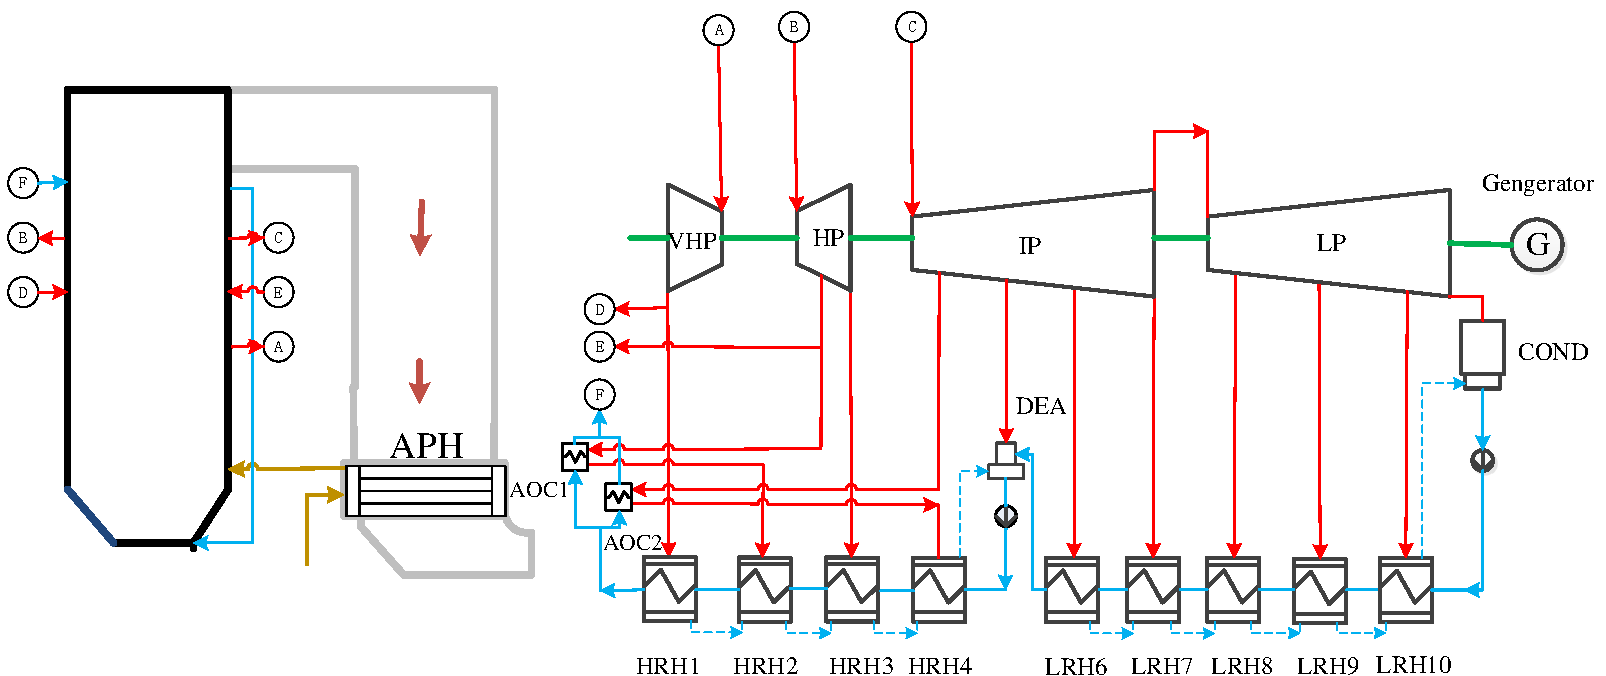
\includegraphics[width=0.9\textwidth]{fig/reference_system}
\caption{Schematic of the reference system} 
\label{fig:reference_system}
\end{figure}
%从参考系统的锅炉虽然仍然采用Π型布置,但其内部受热面和传统一次再热锅炉有较大区别。
Furnace layout shown in Fig~\ref{fig:boiler_surface}, the boiler furnace is composited by the membrane wall, along flue gas flow direction lays low-temperature superheater (Lts) screen tube, cold segment of high-temperature first reheater (Csf), cold segment of high-temperature second reheater (Csf), High temperature super-heater (Hts), hot segment of high-temperature first reheater (Hsf), hot segment of high-temperature second reheater (Hss).
After Hsf and Hss the flue gas channel is divided into the front-duct flue and the back-duct flue. The front duct arranges low-temperature first reheater (Ltfr) and the front-duct economizerz (Feco), the back duct arranges a low-temperature second reheater (Ltsr) and back-duct economizer (Beco). The rear flue is equipped with an air preheater(APH).
% 从锅炉受热面布置可以看出,锅炉主要受热面布置在炉膛之中,而水平烟道和竖井烟道中仅布置有空气预热设备。所以锅炉可以分成两部分:炉膛内完成水/蒸汽吸热的boiler,和尾部烟道内 完成空气预热的APH。
\begin{figure}[htbp]
\centering
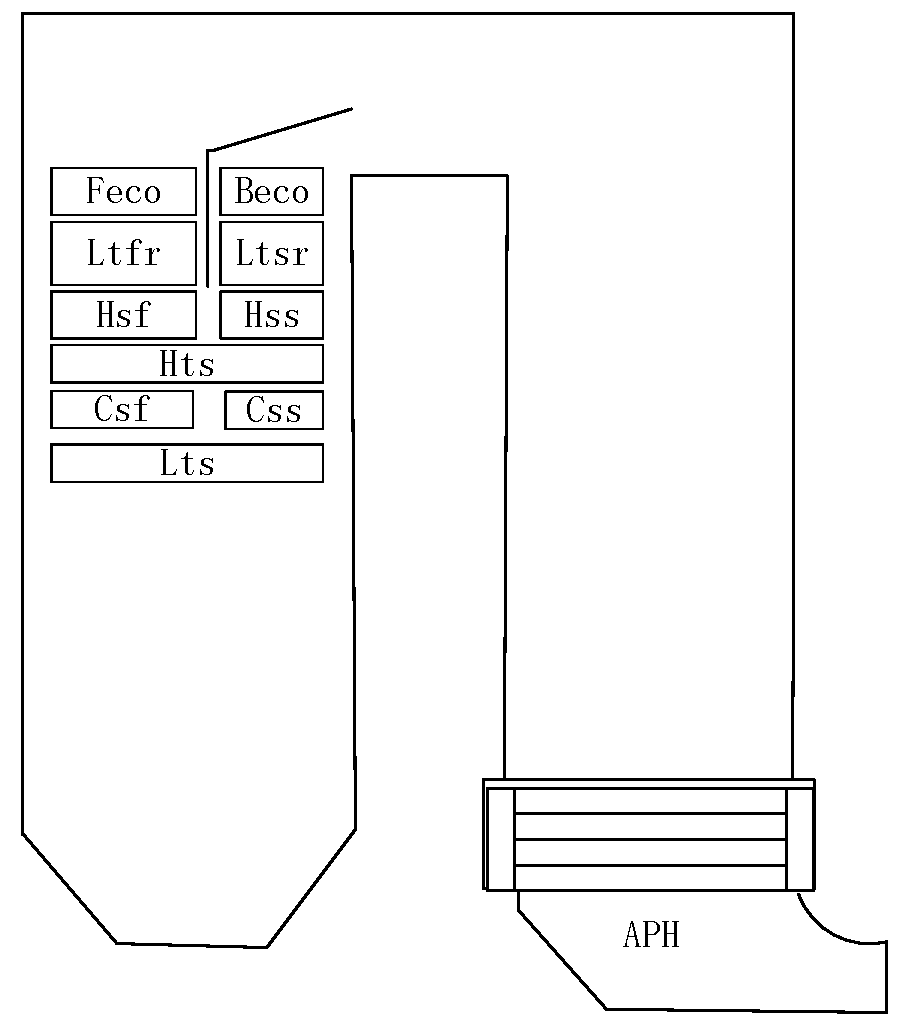
\includegraphics[width=0.5\textwidth]{fig/boiler_surface}
\caption{Boiler internal heat exchangers layout} 
\label{fig:boiler_surface}
\end{figure}


The main  parameters of the reference system are shown in Table~\ref{tab:ref input}.

\begin{table}[htbp]
\caption{The main input parameter of reference system }
\label{tab:ref input}
\centering
\begin{tabular}{lll}
\toprule 
Items & Unit & Value\tabularnewline
\midrule
 Live steam mass flow rate 	    	&t/h 			&2533 \\
 Live steam pressure 		    	&bar 			&310\\
 Live steam temperature		     	&$^\circ$C		&600		\\
 First reheat steam pressure    	&bar			&100.9		\\
 First reheat steam temperature  	&$^\circ$C		&610		\\
 Second reheat steam pressure    	&bar			&30.8		\\
 Second reheat steam temperature 	&$^\circ$C		&610		\\
 Power generation output 			&MW				&1000		\\
\bottomrule
\end{tabular}	
\end{table}
Table 2 gives the temperature profiles and exergy efficiency of regenerative heaters and the air preheater, revealing the energy match level of heat exchangers.
For the air preheater, the temperature of flue gas at the inlet of the air preheater is 376$^\circ$C under THA condition, while the temperature of the air to be heated by the flue is 25$^\circ$C, leading to the exergy loss of 27.17\,MW. The temperature difference of the air preheater is calculated to be 72$^\circ$C, and average temperature of the air is 177$^\circ$C, causing the exergy efficiency of 77.16\%.
\begin{table}[htbp]
\caption{fluid parameters of heat exchangers and air preheater}
\label{tab:reheater parameter}
\centering
\begin{tabular}{llll}
\toprule 
\multirow{2}{2cm}{Components} &\multirow{2}{2.7cm}{Hot fluid temperature($^\circ$C)}  & \multirow{2}{3.2cm}{Cold fluid temperature ($^\circ$C)}&\multirow{2}{2.5cm}{LMTD ($^\circ$C)}\tabularnewline
&&&\tabularnewline
\midrule
APH  &  376.00 	& 23.00  & 72.4\tabularnewline
AOC1 &   526.56 & 304.51 & 69.75\tabularnewline
AOC2 &  527.48 	& 304.51 & 60.81\tabularnewline
HRH1 &   417.07 & 273.62 & 10.64\tabularnewline
HRH2 &   314.53 & 240.73 & 10.77\tabularnewline
HRH3 &   434.54 & 205.89 & 12.68\tabularnewline
HRH4 &   316.51 & 186.48 & 6.88\tabularnewline
LRH6 &  394.01 	& 140.46 & 13.19\tabularnewline
LRH7 &   313.17 & 104.49 & 15.87\tabularnewline
LRH8 &   191.84 & 82.42  & 9.82\tabularnewline
LRH9 &   116.61 & 59.25  & 10.03\tabularnewline
\bottomrule
\end{tabular}
\end{table}

Compared with the air preheater, the regenerative heaters have lower logarithm mean temperature difference (LMTD).
However, it is found that the temperature difference between the hot and cold stream at the inlet high temperature regenerative heaters is also relatively large, which causes irreversible loss. To reduce the superheat degree of the 2nd and 4th extractions and to heat feedwater, two additional outer steam coolers are installed.
Results show that the inlet temperature difference of HRH2 and HRH4 is greatly reduced, and the exergy efficiency is improved correspondingly.
However, the inlet temperature difference between the cold and hot stream of other high temperature regenerative heaters remains very high.
Moreover, because of the material restriction of the water wall, the temperature of feedwater at the inlet of boiler is restricted to 315$^\circ$C. 
In the reference system, the first extraction has to be throttled to ensure the temperature of feedwater not exceeding the restriction.
The pressure of the first extraction is throttled from 106.70 bar to 88.56 bar, and the temperature is decreased from 425.60$^\circ$C to 413.77$^\circ$C. The throttling of the first extraction will certainly cause extra irreversible loss.
%2.2
\subsection{Proposal of a novel system with EAPH and LPE}
\label{sub2:prop novel sys}

The  layout of the optimization system is presented in Fig~\ref{fig:novel_system}.
In the optimization system, the air is not heated by flue gas in the conventional air preheater, and 8 new air preheaters (APH1\-APH8) using several extractions to heat the air is adopted.
The new air preheater is similar with regenerative heaters in function.
As shown in Fig~ the extracted steam is sent to the regenerative heater to heat the condensate or feedwater, and then the drainage from the air preheater joins with that of corresponding regenerative heater.
It should be mentioned that not all the extractions are available for air heating
For the last two stage extractions, their pressure is much lower than barometric pressure which makes it extremely difficult to maintain such low pressure environment inside the heat exchangers, and APH8 shall be shut down under low load for the same reason.
Besides, to reduce the superheat degree of extractions entering the heat exchangers and to improve the air temperature, four additional outer steam coolers (AOC1- AOC4) are installed at the outlet of APH1.
Since extractions from the 2nd to the 5th have superheat degree, they are sent to AOCs in the order of temperature level.
For example, the 2nd extraction has the highest temperature, and is applied to heat the air in the 1st AOC, and then the cooled steam from AOC1 is sent to HRH2 and air APH2 to heat the water and air respectively.   

\begin{figure}[htbp]
\centering
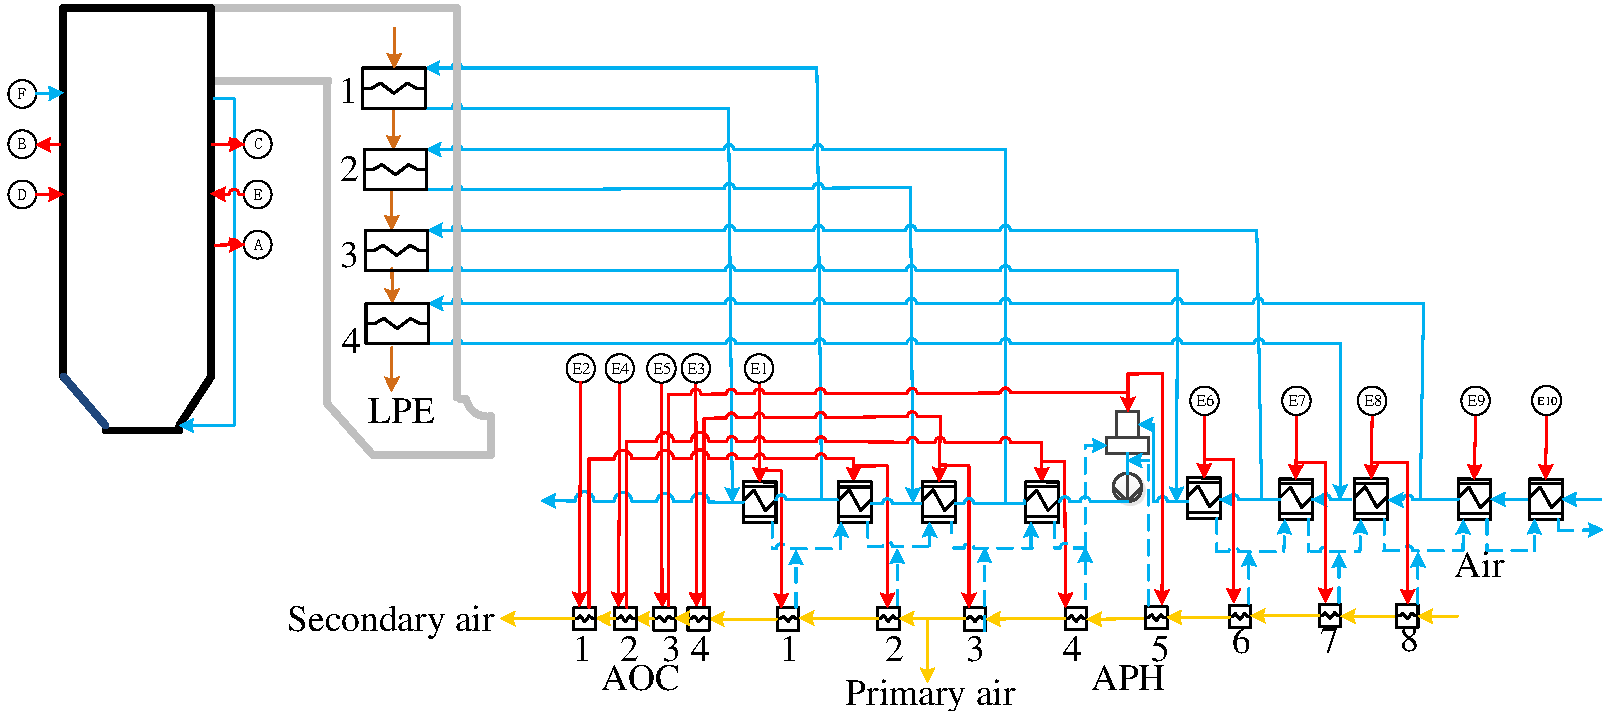
\includegraphics[width=0.9\textwidth]{fig/novel_system}
\caption{Schematic of the novel system} 
\label{fig:novel_system}
\end{figure}

\begin{figure}[htbp]
\centering
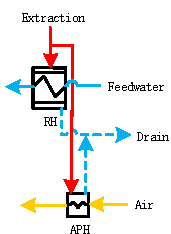
\includegraphics[width=0.3\textwidth]{fig/extraction_heat_APH}
\caption{Process flow diagram of RH and APH} 
\label{fig:extraction_heat_APH}
\end{figure}
As shown in Fig~\ref{fig:novel_system}, the flue gas at the outlet of economizer is utilized to heat the condensate and feed water by four LPEs, which are paralleled to HRH2, HRH4, LRH6, and LRH8 respectively. 
Part of the condensate and feed water at the inlet of regenerative heater are sent to the LPE, then the heated water join with the main feedwater/condensate. 
Considering the acid dew point temperature, the flue gas temperature at the outlet of the last LPE is set 95℃. 
The temperature of heated water from LPE is set little higher than the feedwater from the corresponding regenerative heater.%

\section{Model establishment and thermodynamic evaluation} % (fold)
\label{sec3:modle est and eval}
\subsection{Model description and system analysis method} % (fold)
\label{ssub:model_establishment_and_system_analysis_method}

\subsubsection{Model establish method and main assumption}
\label{ssub3:modle description}
In this paper, the thermodynamic cycle of the thermal system under different loads are simulated with EBSILON® Professional for its flexibility and level of detail. 
EBSILON is a power plant simulation tool which can calculate thermodynamic quantities. 
The simulation model gives the detailed data with high degree of reliability to calculate the thermodynamic state.
EBSIOLON's simulation and parameter calculation of the equipment is based on experimental characteristics of units during the process of modeling design and off-design conditions.
However, only some characteristic curves of turbine can actually be obtained, while boiler and heat exchanger data cannot be obtained, which can only use the system built-in data as an alternative.
It’s needed to assume that the difference between the built-in data and the actual data to meet the error requirements.
The following assumptions need to be made in order to be able to simulate correctly.
\begin{enumerate}[(1)]
\item Both novel and reference systems are operated in stable condition
\item The thermal efficiency of the equipment is calculated from the thermal balance of the input and output parameters of the components, assuming that the calculation error requirement can be met.
\item According to the heat map, set the upper and lower end difference of the heat exchanger as a fixed value, and do not change among different condition.
\item  Do not take the pips' complexity and equipment’s installation difficulty of the novel system as consideration.
\end{enumerate}




\subsubsection{System analysis method} %(fold)
\label{ssub3:analsys method} 
%为了能够对优化系统与参考系统进行评估,揭示系统优化的内在机理,本文引入热力学第二定律的分析方法即用分析方法。
Exergy analysis, is adopted to reveal the location, the magnitude and the sources of thermodynamic inefficiencies of the unit.
Usually, exergy loss and exergy efficiency are chosen as evaluation indices of the thermal system or an individual component, 
The general exergy balance of component can be expressed in the following form:
\begin{equation}
\label{equation:1}
\dot{I}=\sum\dot{E}{}_{in}-\sum\dot{E}{}_{out}+\sum\dot{W}{}_{in}-\sum\dot{W}{}_{out}
\end{equation}
Exergy efficiency can be calculated in the following form:
\begin{equation}
\label{equation:2}
\eta=\frac{\dot{E}{}_{earned}}{\dot{E}{}_{cost}}
\end{equation}
For different equipment under stable operating conditions, equation~\ref{equation:1}~\ref{equation:2} have different forms as shown in Table~\ref{tab:exergy equation}~\cite{Aljundi2009Energy}
For flue gas, air, water and steam, the specific exergy can be calculated by equation~\ref{equation:3}.

\begin{equation}{}
\label{equation:3}
e=h-h_{0}-T_{0}\left(s-s_{0}\right)
\end{equation}
Then the total exergy rate associated with fluid stream becomes:
\begin{equation}
\dot{E}=\dot{m}e=\dot{m}\left[h-h_{0}-T_{0}\left(s-s_{0}\right)\right]{}
\end{equation}
The fuel specific exergy is calculated as[?]: 
\begin{equation}
e_{fuel}=LHV\left(1.0064+0.1519\frac{H}{C}+0.0616\frac{O}{C}+0.0429\frac{N}{C}\right)
\end{equation}
Where LHV refer to lower heating value of fuel, C, H, O, N refer to mass fractions of carbon, hydrogen, oxygen, nitrogen by element analysis.
\begin{table}
\caption{Exergy analysis equations for plant components}
\label{tab:exergy equation}
\centering
\begin{tabular}{lll}
\toprule 
 & Exergy destruction rate  & Exergy efficiency\tabularnewline
\midrule
Boiler & $\dot{I}_{boiler}=\dot{E}{}_{fuel}+\dot{E}{}_{in}-\dot{E}{}_{out}$ & $\eta_{\uppercase\expandafter{\romannumeral2},boiler}=\frac{\dot{E}{}_{out}-\dot{E}{}_{in}}{\dot{E}{}_{fuel}}$\tabularnewline
Pump & $\dot{I}_{pump}=\dot{E}{}_{in}-\dot{E}{}_{out}+\dot{W}{}_{pump}$ & $\eta_{\uppercase\expandafter{\romannumeral2},pump}=1-\frac{\dot{I}_{pump}}{\dot{W}{}_{pump}}$\tabularnewline
Heater & $\dot{I}_{heater}=\dot{E}{}_{in}-\dot{E}{}_{out}$ & $\eta_{\uppercase\expandafter{\romannumeral2},heater}=1-\frac{\dot{I}_{heater}}{\dot{E}{}_{in}}$\tabularnewline
Turbine & $\dot{I}_{turbine}=\dot{E}{}_{in}-\dot{E}{}_{out}-\dot{W}{}_{el}$ & $\eta_{\uppercase\expandafter{\romannumeral2},turbine}=1-\frac{\dot{I}_{turbine}}{\dot{E}{}_{in}-\dot{E}{}_{out}}$\tabularnewline
Condenser & $\dot{I}_{condenser}=\dot{E}{}_{in}-\dot{E}{}_{out}+\dot{W}{}_{p}$ & $\eta_{\uppercase\expandafter{\romannumeral2},boiler}=\frac{\dot{E}{}_{out}}{\dot{E}{}_{in}+\dot{W}{}_{p}}$\tabularnewline
Cycle & $\dot{I}_{cycle}=\sum_{all}\dot{I}_{i}$ & $\eta_{\uppercase\expandafter{\romannumeral2},cycle}=\frac{\dot{W}{}_{net,out}}{\dot{E}{}_{fuel}}$\tabularnewline
\bottomrule
\end{tabular}
\end{table}

\subsection{Thermodynamic performance evaluation} % (fold)
\label{sub:Thermodynamic_evaluation}
Based on the analysis of the reference system, the temperature difference of the heat exchangers is very high and exergy efficiency is rather low.
Using turbine extractions to heat air can realize the reduce the heat transfer temperature difference and improve efficiency. 
The economizer outlet flue gas is used to heat low-temperature economizer can also reduce the loss of regenerative system.
% In order to complete the heat balance calculation of the thermodynamic system, the key parameters in the novel system need to be set.
% The novel system’s parameters are based on reference system, so the main parameters must be the same. The main parameters settled are including: superheat steam’s mass flow, pressure and temperature; First/second reheater’s inlet and outlet pressure and temperature; Turbine Exhaust pressure and temperature; turbine extraction’s pressure and temperature/ specific enthalpy etc. The main parameters settled under THA situation can be found in Table 1 and Table 4 . 
% 对于新旧系统表格的热力参数进行分析,下面这段话太少



\begin{table}
\caption{Thermodynamic performance of the reference and novel systems}
\label{table:thermal performance compare}
\centering
\begin{tabular}{p{7.5cm}p{1.75cm}p{1.75cm}}
\toprule 
Items & Reference system & Novel system\tabularnewline
\midrule
Net generating power (MW) & 999.10 & 1011.19\tabularnewline
Generating efficiency (\%) & 47.69 & 48.73\tabularnewline
Addition in generating efficiency (\%) &  & 1.04\tabularnewline
Standard coal consumption rate (g/kWh) & 257.59 & 252.10\tabularnewline
Reduction in standard coal consumption rate (g/kWh) &  & 5.49\tabularnewline
Exergy efficiency (\%) & 46.51 & 47.52\tabularnewline
Addition in generating efficiency (\%) &  & 1.01\tabularnewline
\bottomrule
\end{tabular}
\end{table}
% 根据用损失对比表从新进行分析,从为什么锅炉空预器效率提高,其他不变或者降低说起
The results of exergy analysis of the optimization system are presented in Table~\ref{table:system exergy campare}. 
It is found that the optimization system has an improvement in exergetic performance.
 The total exergy loss of the cascaded utilization system is 1096.52 MW, which is 32.28 MW lower than the original. 
 The new system also brings the improvement from 46.98\% to 47.99\%. 
 Results show that the exergy loss of boiler is 855.72 MW, leading to the increment of exergy efficiency by 0.18\%. In addition, there is almost no change of the exergy parameters of the steam turbines, generator and condenser. 
 For the air heating system and regenerative system, great change happens compared with the formal system, and detailed analysis will be carried out next.

Through the analysis of the reference system and the optimization system, it can be seen that the exergy efficiency of the optimization system is improved and the exergy loss is reduced.
Comparing the proportion of different components in the total exergy loss between the two systems, we can see that in addition to the turbine, the exergy loss of all components is reduced. 
Among them, the air preheating system efficiency is the most obviously improved,to 38.94\%.


\begin{table}
\caption{Systems' exergy destruction rate comparison }
\label{table:system exergy campare}
\centering
\begin{tabular}{lll}
\toprule 
Items & Reference System\,(MW) & Novel System\,(MW)\tabularnewline
\midrule 
Boiler(without AP) & 883.26 & 872.22\tabularnewline
Turbine & 63.33 & 63.97\tabularnewline
Air Preheater  & 27.39 & 16.55\tabularnewline
Regenerative system & 22.53 & 21.56\tabularnewline
Other & 131.03 & 142.42 \tabularnewline
Total & 1116.72 & 1127.54\tabularnewline
\bottomrule
\end{tabular}
\end{table}



\begin{table}
\label{table:extraction compare}
\caption{Systems' extractions comparison}
\begin{centering}
\begin{tabular}{llll}
\toprule 
\multirow{2}{*}{Extractions} & \multirow{2}{2.5cm}{Reference system (kg/s)} & \multicolumn{2}{c}{Novel system (kg/s)}\tabularnewline
\cmidrule{3-4} 
 &  & to RHs & to APHs\tabularnewline
\midrule
1st & 54.47 & 43.79 & 15.42\tabularnewline
2nd & 52.18 & 18.52 & 13.5\tabularnewline
3rd & 37.86 & 31.71 & 14.62\tabularnewline
4th & 20.53 & 5.66 & 9.5\tabularnewline
5th & 11.95 & 9.78 & 5.67\tabularnewline
6th & 19.94 & 9.88 & 7.83\tabularnewline
7th & 30.19 & 14.16 & 12.85\tabularnewline
8th & 16.31 & 3.11 & 27.1\tabularnewline
9th & 18.93 & 18.93 & 0\tabularnewline
10th & 20.61 & 20.6 & 0\tabularnewline
Total & 282.97 & 176.14 & 106.49\tabularnewline
\bottomrule
\end{tabular}
\par\end{centering}
\end{table}
% 下面两段话需要根据图修改
The variation of mass flow rate of extractions is presented in Fig 6.
 Mass flow rate of the 1st, 3rd, 5th and 8th extractions of the optimization system is more than that of the base model, and the rest extractions except the last two, has the opposite variation. 
 The impact of system optimization on extraction is twofold. 
 Air is heated by extractions, which will cause an increment in mass flow. 
 And the use of LPE can saves extractions.so the total extraction keeps unchanged.
 Turbine total extraction steam volume change affect its exergy efficiency by 2.03\%.

The air is heated by the staged air preheaters and additional outer steam coolers in the cascaded utilization system.
 It can be seen from Table 5 that the total exergy loss of the air heating system is 16.35 MW, 10.82 MW lower than that of the original air preheater which is 27.17 MW. 
 Fig 7 shows that the exergy efficiency of APHs and AOCs is higher than 82\%, except APH8.
 For the air preheaters, the improvement in performance results from more reasonable energy utilization and the heat transform method. 
 In the conventional air preheater, the air is heated by high temperature flue gas through convection. 
 The working principle of the staged air preheaters in the optimization system is the same as regenerative heaters. 
 The superheated vapor is firstly cooled to saturated steam through convection, then to saturated water through phase change heat transfer, and the latter process accounts for the main part. 
 In this case, the temperature difference is greatly reduced, causing the improvement in performance.

\begin{figure}[htbp]
\centering
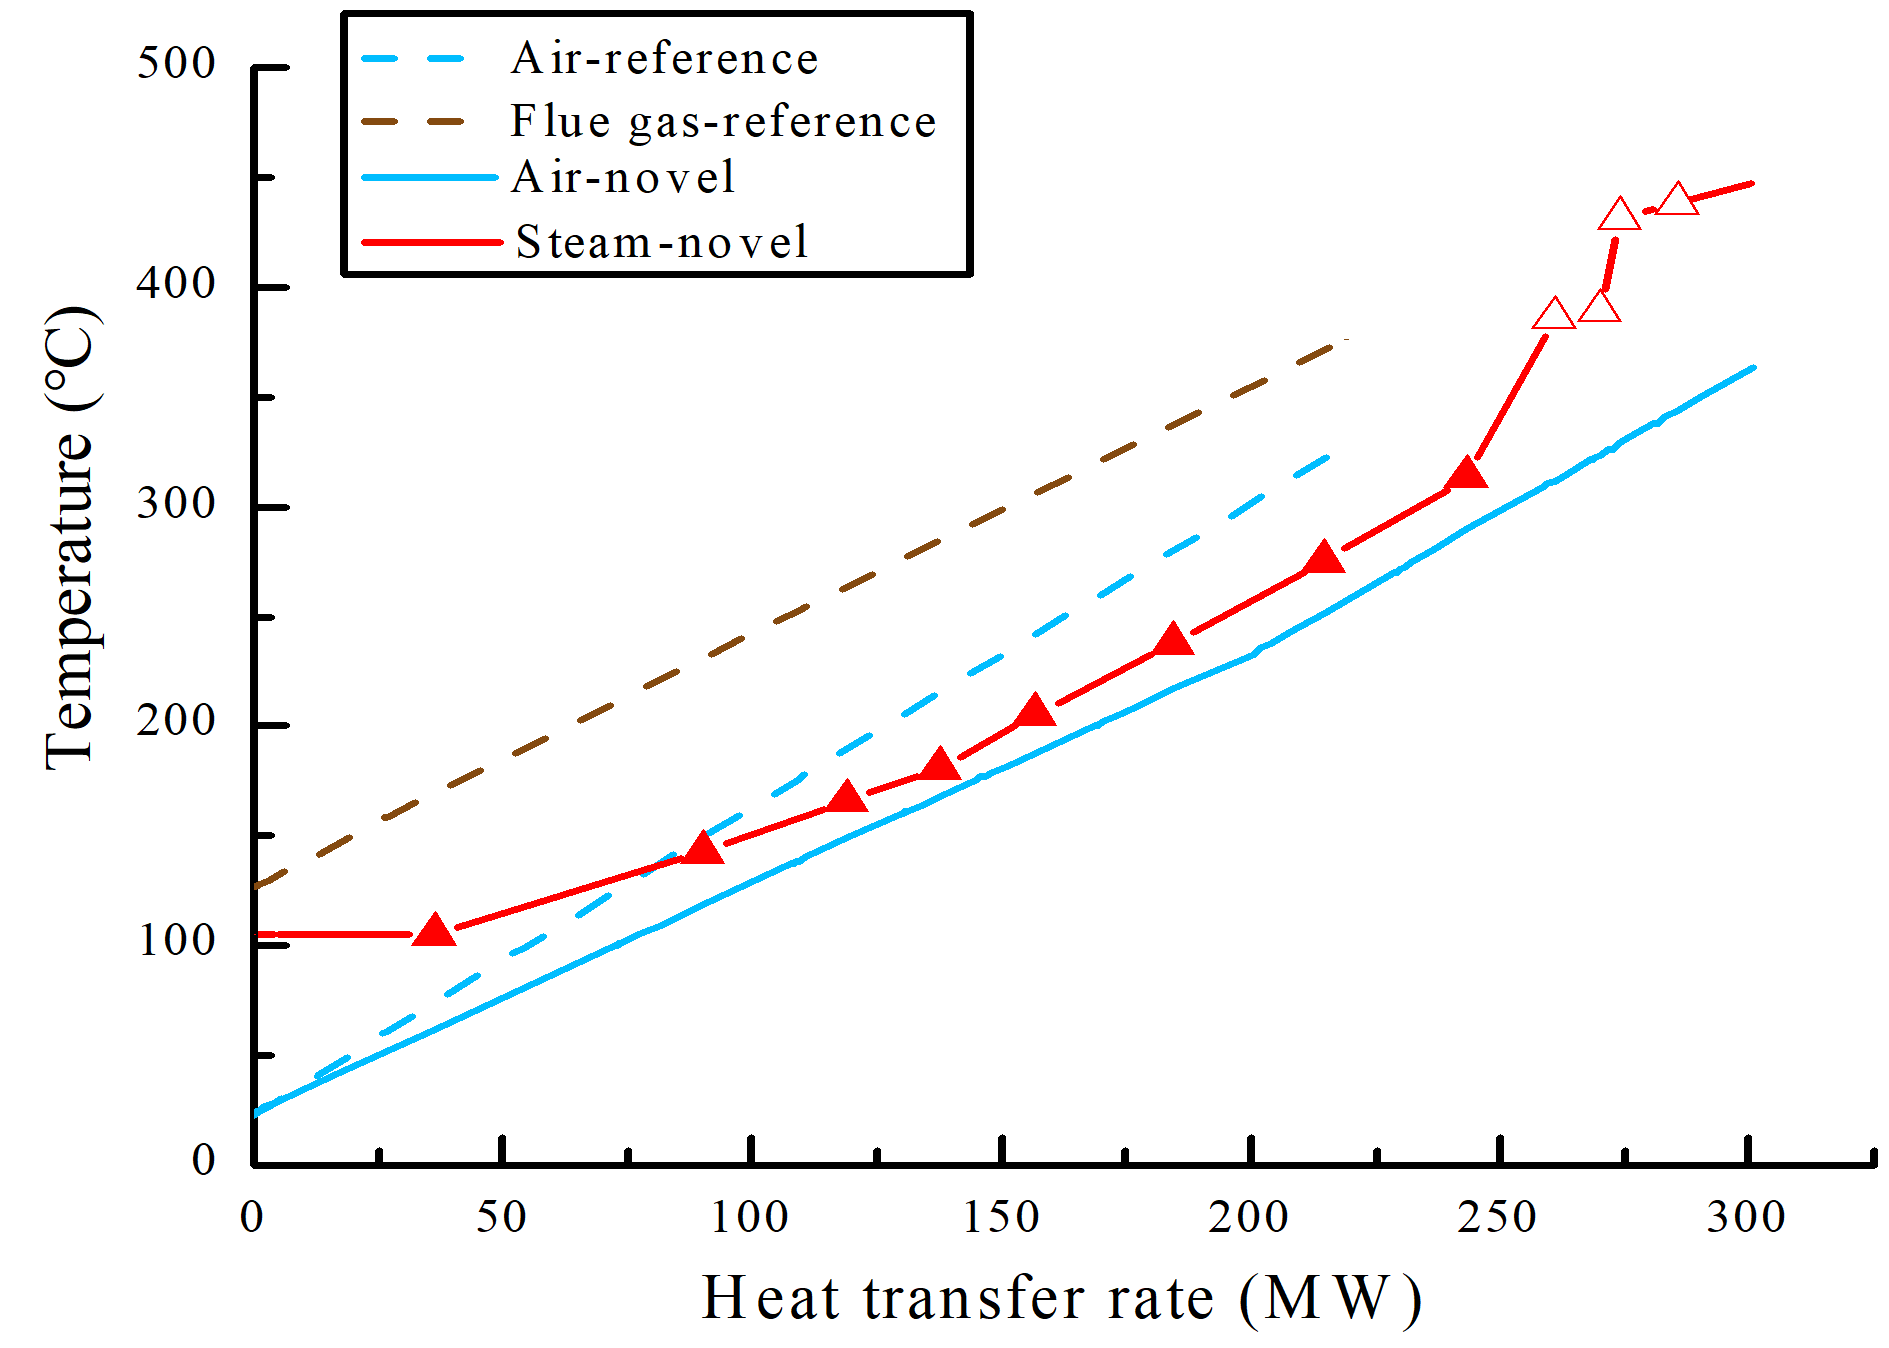
\includegraphics[width=0.6\textwidth]{fig/APH_temper_compare.tif}
\caption{T-q diagram of Air preheat subsystems} 
\label{fig:APH_temper_compare}
\end{figure}

\begin{figure}[htbp]
\centering
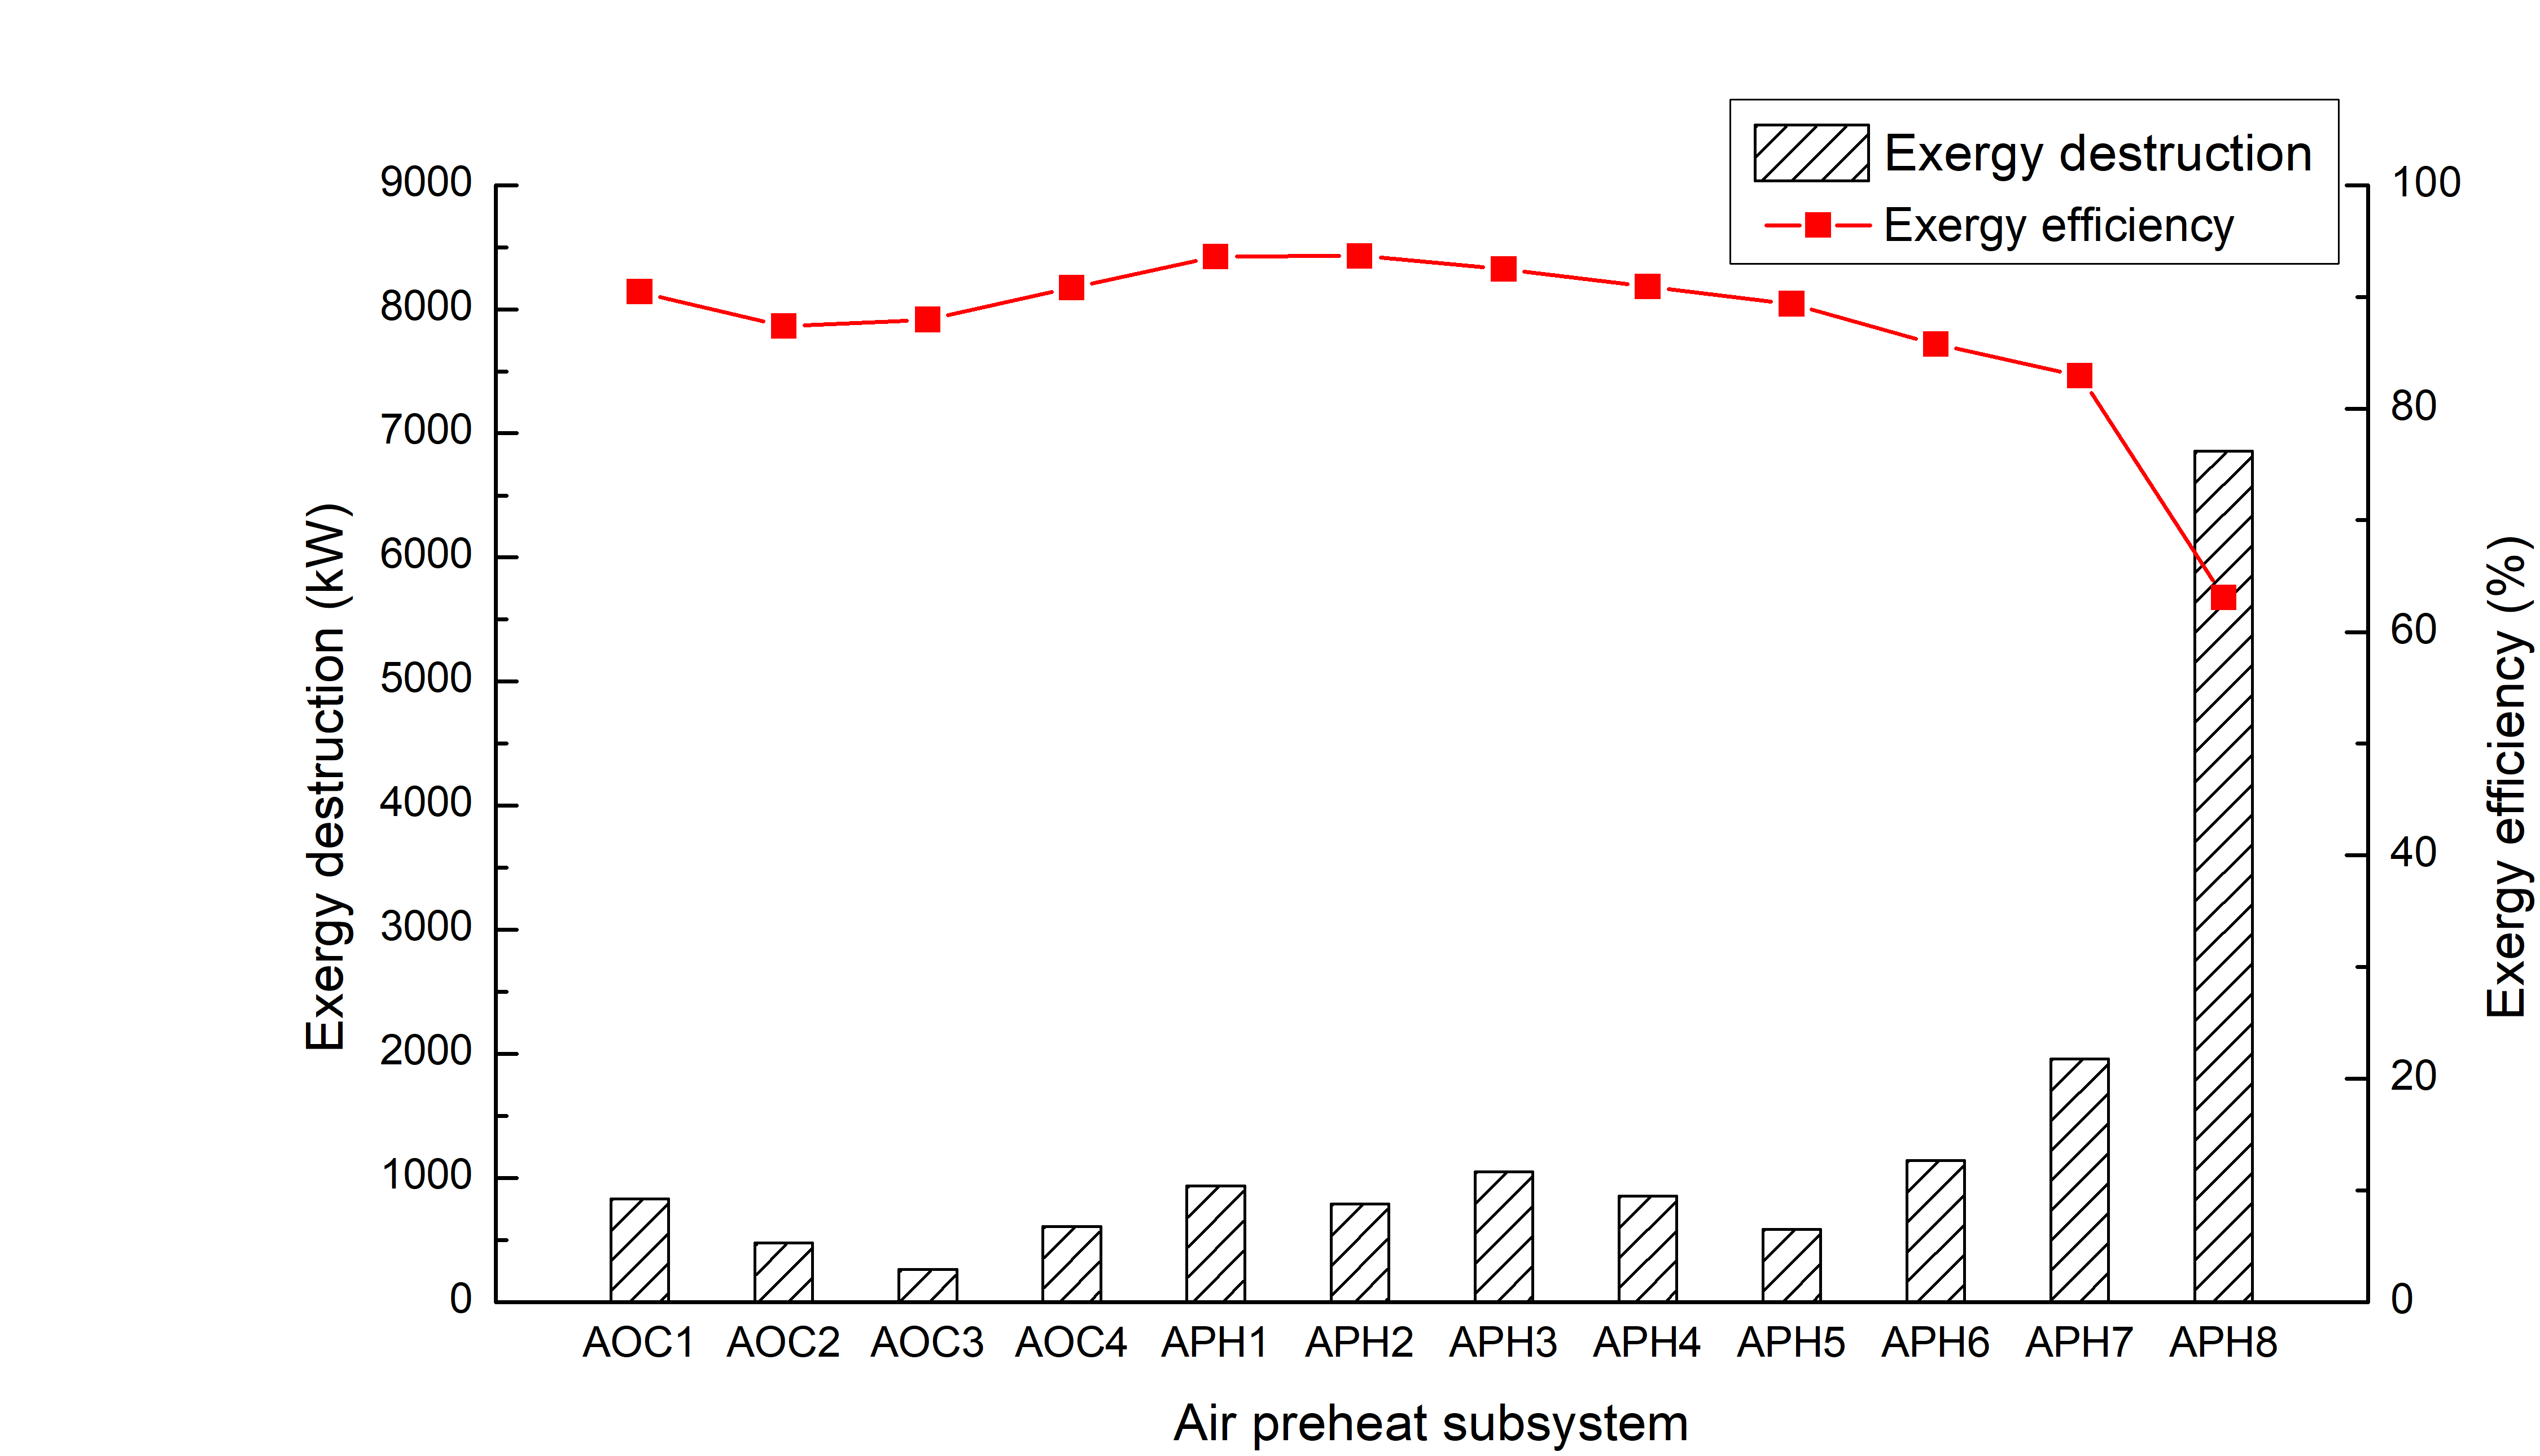
\includegraphics[width=0.6\textwidth]{fig/novel_APH_exergy.tif}
\caption{Exergy destruction and efficiency of air preheat subsystem of novel system} 
\label{fig:novel_APH_exergy}
\end{figure}

% subsubsection subsubsection_name (end)
\section*{References}
\bibliographystyle{elsarticle-num}

\bibliography{bib/reference.bib}


\end{document}

\endinput
\%\%
\%\% End of file `article.tex'.
